\documentclass{article}
\usepackage[UTF8]{ctex}
\usepackage{geometry}
\usepackage{multirow}
\usepackage{natbib}
\geometry{left=3.18cm,right=3.18cm,top=2.54cm,bottom=2.54cm}
\usepackage{graphicx}
\pagestyle{plain}	
\usepackage{setspace}
\usepackage{enumerate}
\usepackage{caption2}
\usepackage{datetime} %日期
\renewcommand{\today}{\number\year 年 \number\month 月 \number\day 日}
\renewcommand{\captionlabelfont}{\small}
\renewcommand{\captionfont}{\small}
\begin{document}

\begin{figure}
    \centering
    
\includegraphics[width=8cm]{upc.png}

    \label{figupc}
\end{figure}

	\begin{center}
		\quad \\
		\quad \\
		\heiti \fontsize{45}{17} \quad \quad \quad 
		\vskip 1.5cm
		\heiti \zihao{2} 《计算科学导论》个人职业规划
	\end{center}
	\vskip 2.0cm
		
	\begin{quotation}
% 	\begin{center}
		\doublespacing
		
        \zihao{4}\par\setlength\parindent{7em}
		\quad 

		学生姓名:\underline{\qquad  王春祥 \qquad \qquad}

		学\hspace{0.61cm} 号:\underline{\qquad 1906050123 \qquad}
		
		专业班级:\underline{\qquad 计算1903班 \qquad  }
		
        学\hspace{0.61cm} 院:\underline{计算机科学与技术学院}
% 	\end{center}
		\vskip 1.5cm
		\centering
		\begin{table}[h]
            \centering 
            \zihao{4}
            \begin{tabular}{|c|c|c|c|c|c|c|c|c|}
            % 这里的rl 与表格对应可以看到,姓名是r,右对齐的;学号是l,左对齐的;若想居中,使用c关键字。
                \hline
                \multicolumn{5}{|c|}{分项评价} &\multicolumn{2}{c|}{整体评价}  & 总    分 & 评 阅 教 师\\
                \hline
                自我 & 环境 & 职业 & 实施 & 评估与 & 完整性 & 可行性 &\multirow{2}*{} &\multirow{2}*{}\\
                分析& 分析& 定位 & 方案 & 调整 & 20\% & 20\% & ~&~ \\\            
                10\% & 10\% & 15\% & 15\% & 10\% & &  &~ &~\\
                \cline{1-7} 
                & & & & & & & ~&~ \\
                & & & & & & & ~&~ \\
                \hline      
            \end{tabular}
        \end{table}
		\vskip 2cm
		\today
	\end{quotation}

\thispagestyle{empty}
\newpage
\setcounter{page}{1}
% 在这之前是封面,在这之后是正文
\section{自我分析}
	自我分析即对自己进行全方位、多角度的分析,目的是认识自己、了解自己。只有认识了自己,才能对自己的职业做出正确的选择,才能选定适合自己发展的职业生涯路线,才能对自己的职业生涯目标做出最佳抉择。\par
	自我分析包括:\par
\subsection{自然条件}
本人性别男,现在21岁,身体的素质正常偏下,精力的充沛时间主要分布在傍晚和晚上,需要通过锻炼来增强自己的体质,目前健康状况处于健康和亚健康之间,但不是长期状态,未来可以胜任一些中高强度工作。现在居住地为山东省临沂市沂南县,未来职业目标是向一二线城市发展。
\par
\subsection{性格分析}
关于性格分析,我引入一部分关于自身的霍兰德测试结果:
\begin{figure}[h!]
\centering
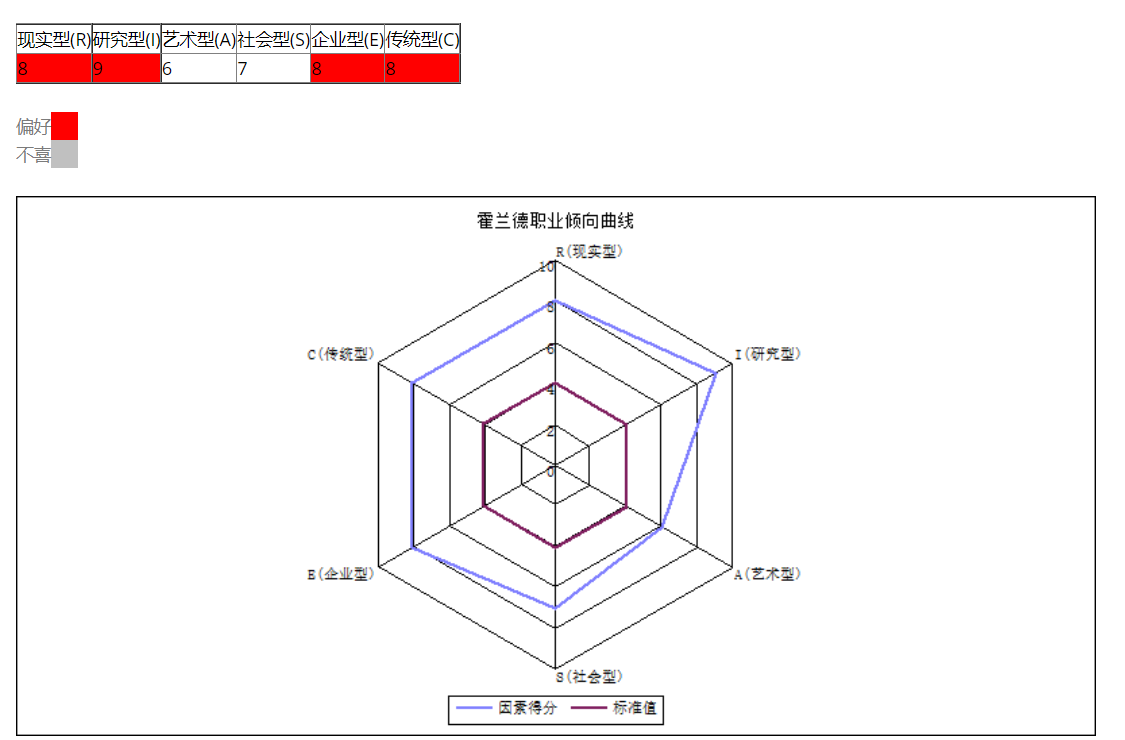
\includegraphics[width=0.95\textwidth]{hld}
\caption{霍兰德测试得分结果}
\label{fig:hld}
\end{figure}
\par
根据霍兰德测试,我的职业兴趣代码是:IRE , IER , IRC , IEC , ICR , ICE
\par
IRE:IRE适合的典型专业有:经济学、材料成型及控制工程、电气工程及其自动化、物理学、化学、生物科学、生物化学、材料化学、微电子学、轻化工程、采矿工程、民用工程、地理学、地质学、数学、计算机科学、统计学、人种学、考古学、环境科学、农业工程、计算机工程、电子工程、机械工程、建筑学等。适合的典型职业有:化学家、化验员、化学工程师、纺织工程师、食品技师、渔业技术专家、材料和测试工程师、电气工程师、土木工程师、航空工程师、行政官员、冶金专家、原子核工程师、陶瓷工程师、地质工程师、电力工程师、口腔科医生、牙科医生、公共卫生医师、制图员、测绘师。
\par
IER:IER适合的专业有心理学、气象学、水利工程、农业工程、地理学、经济学、网络工程、管理工程、环境工程、安全工程、财政学、市政规划、工业心理学、工业工程、计算机科学、应用数学等。适合的职业有水利工程师、工业工程师、网络工程师、管理分析师、数据分析师、审计师、工业心理学家、农业工程师、地质工程师、环境工程师、安全员、学校心理师、气象员、实验管理员、领航员、土壤学家、系统工程师、影视技师、仓储工程师、工业治疗师、信息工程师、机械师、药剂师、农业机械师、侦查员、科技作家、软件工程主管、设备工程师、海军军官、工业工程教师、现场工程师等。
\par
IRC:IRC适合的典型专业有:管理科学、冶金工程、金属材料工程、无机非金属材料工程、高分子材料与工程、材料成型及控制工程、过程装备与控制工程、热能与动力工程、电气工程及其自动化、通信工程、计算机科学与技术、生物医学工程、测绘工程、制药工程、交通工程、信息与计算科学、物理学、生物科学类、地质学、地球物理学、大气科学类、理论与应用力学、材料化学、中医学、交通运输。适合的典型职业有:飞机领航员、飞行员、物理实验室技师、文献检查员、农业技术专家、动植物技术专家、生物技师、油管检查员、工商业规划者、矿藏安全检查员、纺织品检验员、照相机修理者、工程技术员、编计算程序者、工具设计者、仪器维修工。
\par
IEC:IEC适合的典型专业有:水利水电工程、计算机科学、软件工程、财政学、财务管理、应用数学。适合的典型职业有:计算机科学家、软件工程师、档案保管员、保险统计员、证券分析师、财务主管。
\par
ICR:ICR适合的典型专业有:药学、制药工程、交通工程、地质学、地球物理学、大气科学、中医学、基础医学、自动化、水文与水资源工程、统计学等。适合的典型职业有:质量检验技术员、药剂师、物理学家、地质学技师、环境工程师、法官、图书馆技术辅导员、计算机科学家、医院听诊员、家禽检查员、水利工程师、理疗师、中医师、公共卫生医师、医疗顾问。
\par
ICE:ICE适合的专业有财政学、水利工程、中文、外国语、人类学、审计学、包装工程、工程管理、图书馆学、信息工程、侦查学等。适合的职业有语言学家、语言教师、人类学家、审计师、包装师、项目经理、图书馆员、网络/数据库工程师、侦探等。
\par
综上所述,我认为霍兰德测试报告只能做一个参考,还需要结合我个人事情情况来做出职业的选择,我认为我比较理性,同时喜欢学习一些新的东西,是一名技术宅,以后可能适合做一名软件工程师或者架构师。
\par
\subsection{教育与学习经历}
(1)高中就读于山东省沂南第一中学,就读期间学习成绩尚可。\par
(2)2019学年就读于中国石油大学(华东)储运与建筑工程学院的建筑学,后在2020年中旬转入计算机科学与技术学院,并一直就读于计算机科学与技术专业。
\par
\subsection{工作与社会阅历}
工作与社会阅历基本为0,之前未参加过有关项目的实习,希望在大四的实习当中获取知识,增加自我社会阅历。
\par
\subsection{知识、技能与经验}
目前所掌握的知识大部分为上课所传授的知识,少部分为自己通过一些博客以及课外书籍所学习的知识,现在基本能够做到网站的搭建与运营,网站前后端的开发以及安卓配套应用的开发。
\par
另外我也参加过相关编程竞赛,通过竞赛将自己课上所学的知识应用于实际,不仅能够提高自我编程能力,同时也能进一步巩固课上所学知识。
\par
\subsection{兴趣爱好与特长}
本人一大兴趣爱好便是编程,我在大一上学期学习C语言时才接触编程,从那之后便对编程产生了兴趣并且从那时起便保持编程的习惯,并且顺利在大一下学期时通过学科特长转入计算机科学与技术专业。
\par
另外的特长方面,我自认为我编程能力尚可,个人在编程实现方面能够比他人更快更好的实现,另外在学习一门新的编程语言时我也比较容易上手。
\par
个人的另一大特长便是好奇心比较强,对一些新的框架、技术或者编程语言比较好奇,所以在日常生活当中我也会学习并尝试一些新的技术。
\section{环境分析}
环境分析主要是评估周边各种环境因素对自己职业生涯发展的影响。每一个人都处在一定的环境之中,职业发展必然要受到所处环境的影响,只有充分了解和把握所处环境的现状、特点、发展变化趋势,才能做到在复杂的环境中避害趋利,使你的职业生涯规划具有实际意义。\par
环境分析包括:\par
\subsection{社会环境分析}
\subsubsection{政治形势}
当前政治形势正位于百年未有之大变局,联合国五常中俄美英法仍然起举足轻重的作用,地区组织发挥一定的影响力。联合国五常中俄美英法仍然起举足轻重的作用,地区组织发挥一定的影响力。国际政治形势在变局中深刻发展,新冠疫情给世界各国带来巨大冲击,逆全球化和单边主义继续酝酿,大国竞争明显升温。
\subsubsection{经济形势}
2021年我国经济总体稳步发展,经济总量规模稳定持续扩大,人均GDP水平继续向高收入国家门槛靠近。2021年前三季度我国GDP增长9.8\%,全年经济增长预计增长8\%以上,高于年初的预期目标,经济运行保持在合理区间。同2019年相比,两年平均增长5.1\% 以上。考虑到价格因素,今年我国GDP总量将超过110万亿元,如果人口增长速度保持在去年的水平,人均GDP将增加到77800元,考虑到人民币升值因素,2021年我国人均GDP将会达到12000美元,距高收入国家门槛值只有半步之遥。
\subsubsection{就业形势}
从整体的大环境来看,就业形势非常严峻。数据显示,2021届全国普通高校毕业生总规模909万,同比增加35万,再创新高。
\par
与此同时,更多海外留学生选择回国找工作,这让今年的职场新人们面临更加激烈的竞争。最新数据显示,2020年,向国内岗位投递简历的海归人才数量较2019年增长了33.9\%。而在今年春节后第二周,随着考研成绩公布,更多应届生流向就业市场,求职人数同比增长143.1\%。
\par
\subsection{家庭环境分析}
% 婚姻状况、经济状况、家人期望、家族传统等。
家庭状态和睦,经济情况中等,家人对于我个人的期望并没有十分明确的限制,仅仅希望我能够凭借自己的本领去选择自己喜欢的职业,无家族传统。对于我选择计算机行业并且在计算机行业内发展,迎接挑战并继续完善自我,恰恰合适。
\par
\subsection{职业环境分析}
计算机行业和其他行业相比技术技术迭代更快,可能每天都会有新的技术出现,同时可能每天都会有新的名词、新的技术和新的架构出现。在未来的一段时间,预计计算机行业会有以下的变化:市场需求不断扩大,越来越多的人参与到计算机行业当中,新技术不断迭代更新,对人才的要求也逐步提高。
\par

\subsection{地域与人际环境分析}
对未来工作的城市我目前还没有一个确切的概念,但是很大概率上我不会选择我的故乡,这里互联网产业发展并不太好,发展的机遇也不会太多。目前个人的想法是到一个互联网产业发达的或正在发展中的城市当中参加工作,这样不仅能够拓宽自己的视野,也同时能够实现自我价值。
% 工作城市的气候水土、文化特点、发展前景;人脉与人际关系等。\par
% \par 
% 图片插入的样例:\par
% \begin{figure}[h!]
% \centering
% 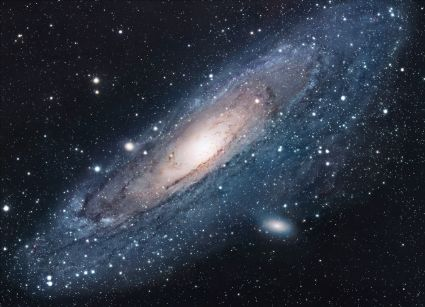
\includegraphics[scale=1.7]{universe}
% \caption{The Universe}
% \label{fig:universe}
% \end{figure}



\section{职业定位}
在准确地对自己和环境做出了分析之后,确定适合自己行业和有实现可能的职业发展目标。职业定位时要注意与自己的自然条件、知识背景、技能特长、性格特点、兴趣爱好是否匹配,考虑与自己所处的环境是否相适应。职业定位决定了职业发展中的行为和结果,是制定职业生涯规划的关键,应当科学合理,具有可行性。\par
职业定位包括:\par

\subsection{行业领域定位与理由}
行业领域定位:软件行业
\par
理由:软件行业符合我现在所学的专业,同时软件开发方向也是我们这个专业培养方案的一个方向,另外个人对这方面的知识了解的比较多,另外这个行业发展前景较好,有着较大的发展空间。
\par
\subsection{职业岗位起点定位与理由}
职业岗位起点定位:软件开发工程师
\par
理由:个人对软件这个方向学习的知识较多,另外软件行业中软件开发工程师的职业前景较好,有较大的发展空间,目前打算是进入企业后先尝试做一段时间的实习生,适应环境,积累经验,拓宽视野,之后根据实际情况决定自己的未来发展方向。
\par
\subsection{职业目标与可行性分析}
\par
% 成果目标、经济目标、能力目标、职务目标等。\par 
\begin{enumerate}[(1)]
	\item 短期目标(大学4年)
	\par
	大学四年的学习生活对于我而言已经过去大半,对于我个人而言只有三个学期,我打算在这剩余的三个学期的时间里,首先学好专业课,打好基础,同时如果有机会就去参加相关公司的实习,以实习的方式提高自我能力,同时将所学知识应用于实际,最后做好毕业设计,完成大学四年的学习时光。
	\item 中长期目标(5-10年)。
	\par
	目前个人打算是优先考虑继续攻读研究生,其次是找工作,所以预计在五到十年的时候我应该在上研究生,在研究生阶段,我会寻找机会,多参加相关公司的实习,并且选好导师,参与到导师的项目,积累更多的经验。
	\par
	在研究生毕业之前寻找合适的工作岗位,未来的想法和环境可能会发生巨大的变化,到时候应当随机应变,对计划做出动态调整,但是上面所说的软件开发工程师依然是一个比较好的选择。
\end{enumerate}
% 这里是简单列表的样例:(如果需要标号自定义或者自动标记数字序号,请自行搜索语法)
% \begin{itemize}
%     \item 简单的列表结构 
%     \item 如这里所示
%     \item 此处仅为样例
%     \item 按需修改和使用
% \end{itemize}


\section{实施方案}
在学校的剩余的三个学期当中,我会踏踏实实的把剩余的专业课学好,为以后的研究生阶段和工作阶段打下牢固的基础,同时如果有机会的话可以去参加相关公司的实习,借实习的机会提高自我工作能力,同时将所学知识应用于实际,进一步巩固所学知识。
\par
关于如何利用现有条件和自身优势以实现职业生涯目标,我认为个人所学的知识大多数知识停留在纸上,缺乏相应的工作经验,在今后应当多参加有关实习,将自己所学的知识应用于实际,发挥个人优势并且进一步提高个人能力。
\par
关于如何克服缺点、弥补不足、增长知识、提高能力以实现职业生涯目标,我认为个人的缺点是做事不够认真仔细,容易犯错,在今后的学习和工作中应当注意这些缺点,正是自己的不足并努力克服,进一步完善自我。
\par
关于如何处理人际关系和发展人脉以实现职业生涯目标,个人认为我自身的人际关系处理能力较弱,在今后的学习和工作途中应当多参加小组项目,学会与他人合作,发展个人人脉。
\par
关于如何处理工作与家庭、生活的关系以实现职业生涯目标,目前暂未考虑到,待到以后做出调整。
\par
关于如何处理释放工作压力、保证身心健康以实现职业生涯目标,我认为在今后的工作中应当合理处理好工作和生活的关系,如果压力过大,则可以通过锻炼或者看电影的方式进行减缓。
% 在明确了职业定位后,要制定实现职业生涯目标的行动方案,不付诸行动,职业目标只能是一种梦想。实施方案是实现职业目标的保证,尽量考虑周全、具有可操作性。\par
% 分析我现有的条件和
% 实施方案可以从以下角度考虑:\par
% \begin{enumerate}[1、]
% 	\item 如何利用现有条件和自身优势以实现职业生涯目标。
% 	\item 如何克服缺点、弥补不足、增长知识、提高能力以实现职业生涯目标。
% 	\item 如何处理人际关系和发展人脉以实现职业生涯目标。
% 	\item 如何处理工作与家庭、生活的关系以实现职业生涯目标。
% 	\item 如何处理释放工作压力、保证身心健康以实现职业生涯目标。
% \end{enumerate}
\par 
% 表格插入样例(三线表):\par
%单元格怎么写?参考第一页打分的表格

% \begin{table}[h]
% 	\centering
% 	\caption{这是科学系的花名册}
% 	\begin{tabular}{rl}
% 		% 这里的rl 与表格对应可以看到,姓名是r,右对齐的;学号是l,左对齐的;若想居中,使用c关键字。
% 		\hline
% 		姓名 & 学号 \\
% 		\hline
% 		张三 & 190704xxxx+++ \\ 
% 		李四 & 190704yyyy \\
% 		王二五 & 190704zzzz\\
% 		\hline
% 	\end{tabular}
% 	\label{table1}
% \end{table}
\section{评估与调整}
由于影响职业生涯规划的因素很多,且大都处于动态变化之中,因此职业生涯规划应定期评估,并根据影响因素的变化和实施结果的情况及时作出调整,这样才能保证其行之有效。\par 
\subsection{评估时间}
一般情况下为一个学期评估一次,经过一个学期的学习之后,个人的能力有所提高,并且行业市场需求也应有所变化,此时根据具体的情况对自我进行评估,并根据目标完成情况调整自我目标。\par
\subsection{评估内容}
% 可以从成果目标、经济目标、能力目标、职务目标等方面总结,确定哪些目标已按预期实现,哪些目标商未达到,对已实现的成果总结经验,对未完成的目标分析原因。\par
可根据自最初设定的目标和实际完成情况进行评价。如果目标完成,则对后期的目标进行细化。反之,则分析目标没有达成的原因,同时结合目标的重要性和完成情况对目标进行评估,决定是否继续执行未完成的目标,如果重要性较高,则继续执行未完成的目标,其余目标进行顺延,反之则放弃未完成的目标,继续执行下一个目标。另外在评估目标完成情况时应当结合自身和实际情况对目标进行调整,使其能够正确引导个人的发展。
\subsection{调整原则}
目前情况下职业规划的大体方向不会发生变化,故职业规划在近两年内不会发生明显的变动,除非有行业环境发生巨大的变化导致个人的发展无法适应行业的发展.
\par
一般情况下调整内容为初期职位变化和近期目标的细化,应当根据市场的需求变化和自身的实际情况以及目标完成情况做出合理的调整。
% 应考虑与自身情况的匹配性、与环境的适应性、操作实施的可行性等。
\par




\end{document}
